\documentclass[11pt]{beamer}
\mode<presentation>
\usepackage[utf8]{inputenc}
\usepackage[T1]{fontenc}
\usetheme{metropolis}
% Define some colors:

\begin{document}
\author{Matthew Schiffman}
\title{Coin-ID}
\subtitle{Grading rare coins using wide and deep neural networks}
\institute{MattSchiffman.com \\
linkedin.com/in/MattSchiffman\\
github.com/someonenamedmatt/coin-ID}
\date{\today}
\setbeamercovered{transparent}
\setbeamertemplate{navigation symbols}
\begin{frame}
	\titlepage
\end{frame}
\begin{frame}
	\frametitle{Motivation}
	\begin{columns}[onlytextwidth]
		\begin{column}{.5\textwidth}
		\begin{itemize}
			\item \$5B market
			\item 2 companies grading 90\% of coins
			\item They only agree on 41\% of grades!
		\end{itemize}
		\end{column}
		\begin{column}{.5\textwidth}
			\begin{figure}
				\centering
				\includegraphics[width=0.5\linewidth]{images/Whole/2000009.jpg}
				\caption{PCGS Graded Coin}
			\end{figure}
		\end{column}
	\end{columns}
\end{frame}
\begin{frame}
	\frametitle{ Model - 76\% Accuracy!}
	\begin{figure}
		\centering
		\includegraphics[height = .8\textheight,width=\textwidth]{images/graph.pdf}
		\label{fig:graph}
	\end{figure}
\end{frame}
\begin{frame}
	\frametitle{Pipeline}
	\begin{columns}[onlytextwidth]
		\begin{column}{.35\textwidth}
			\begin{itemize}
				\item{\alert<2> {Data}}
				\item{\alert<3>{Feature Engineering}}
				\item{\alert<4-6>{Model Selection}}
				\item{\alert<7>{Model Tuning}}
			\end{itemize}
		\end{column}
		\only<7>{\begin{column}{.65\textwidth}
			\begin{itemize}
				\item Balancing Classes
				\item Network Structure (Alexnet, Imagenet, Network in Network)
				\item Regularization
			\end{itemize}
		\end{column}}
		\only<2>{
		\begin{column}{.65\textwidth}
			\begin{itemize}
				\item 600,000 images on EC2 Instances
				\item Separate 5000 image test set
			\end{itemize}
		\end{column}}
		\only<4>{
		\begin{column}{.65\textwidth}
			\centering
			\includegraphics[width = .3\textwidth]{images/Whole/9.jpg}
			\includegraphics[width = .3\textwidth]{images/Whole/1000009.jpg}\\
			\includegraphics[width = .3\textwidth]{images/Whole/2000009.jpg}
			\includegraphics[width = .3\textwidth]{images/Whole/3000009.jpg}
		\end{column}}
		\only<5>{
		\begin{column}{.65\textwidth}
			\centering
			\includegraphics[width = .3\textwidth]{images/Cropped/9.jpg}
			\includegraphics[width = .3\textwidth]{images/Cropped/1000009.jpg}\\
			\includegraphics[width = .3\textwidth]{images/Cropped/2000009.jpg}
			\includegraphics[width = .3\textwidth]{images/Cropped/3000009.jpg}
		\end{column}}
		\only<6>{
		\setbeamertemplate{caption}{\raggedright\insertcaption\par}
		\begin{column}{.65\textwidth}
			\centering
			\begin{figure}
				\centering
				\includegraphics[width = .3\textwidth]{images/distorted.png}
				\label{fig:graph}
				\caption{An image that's been cropped, flipped, and darkened}
			\end{figure}
			\begin{figure}
				\centering
				\includegraphics[width = .3\textwidth]{images/radial.png}
				\label{fig:graph}
				\caption{A radially transformed image}
			\end{figure}
		\end{column}}
		\only<3>{
		\setbeamertemplate{caption}{\raggedright\insertcaption\par}
		\begin{column}{.3\textwidth}
			\begin{figure}
				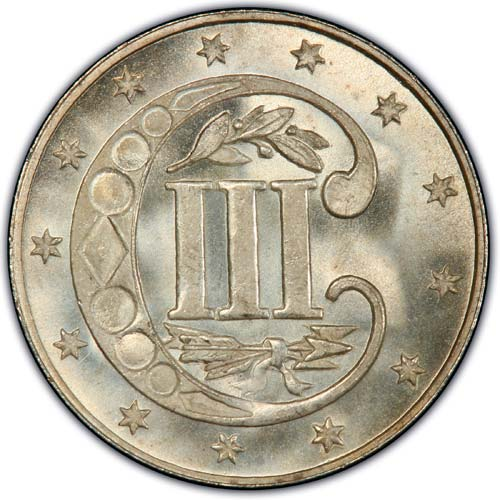
\includegraphics[width=.45\linewidth]{images/3CentSil2-68r.jpg}
				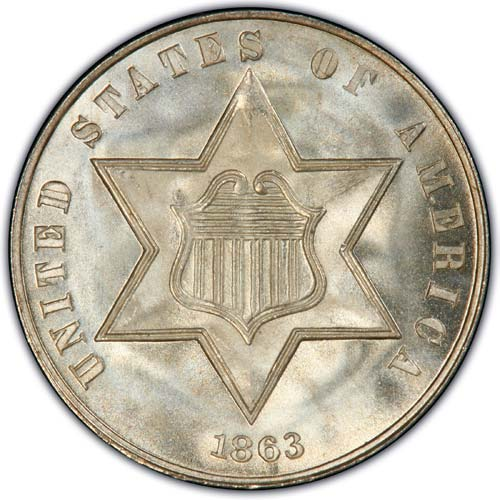
\includegraphics[width=.45\linewidth]{images/3CentSil2-68o.jpg}
				\label{fig:cond3}
				\caption{Mint Condition}
			\end{figure}
			\begin{figure}
				\centering
				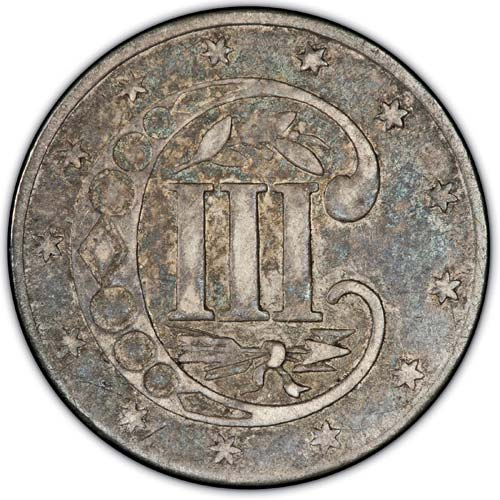
\includegraphics[width=0.45\linewidth]{images/3CentSil2-45r.jpg}
				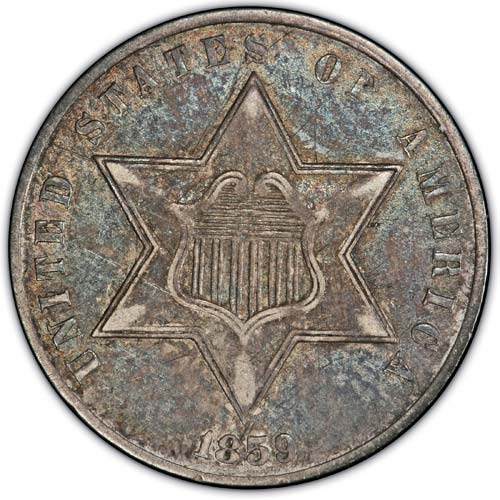
\includegraphics[width=0.45\linewidth]{images/3CentSil2-45o.jpg}
				\caption{Fine}
			\end{figure}
		\end{column}
		\begin{column}{.3\textwidth}
			\begin{figure}
				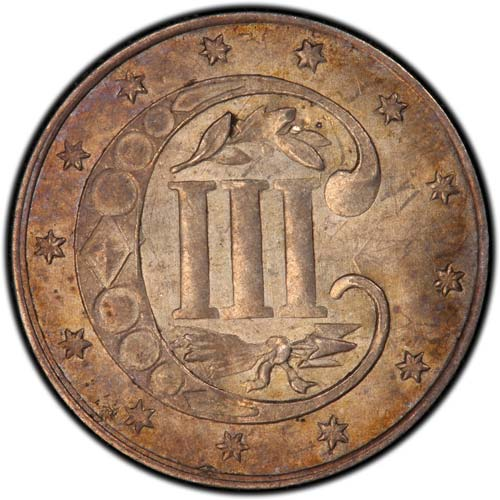
\includegraphics[width=0.45\linewidth]{images/3CentSil2-61r.jpg}
				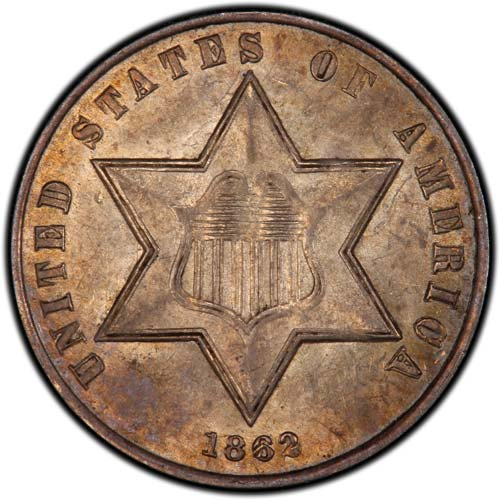
\includegraphics[width=0.45\linewidth]{images/3CentSil2-61o.jpg}
				\label{fig:cond2}
				\caption{About Uncirculated}
			\end{figure}
			\begin{figure}
				\centering
				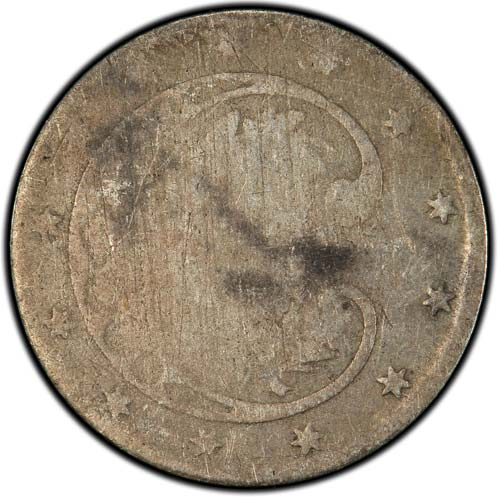
\includegraphics[width=0.45\linewidth]{images/3CentSil2-03r.jpg}
				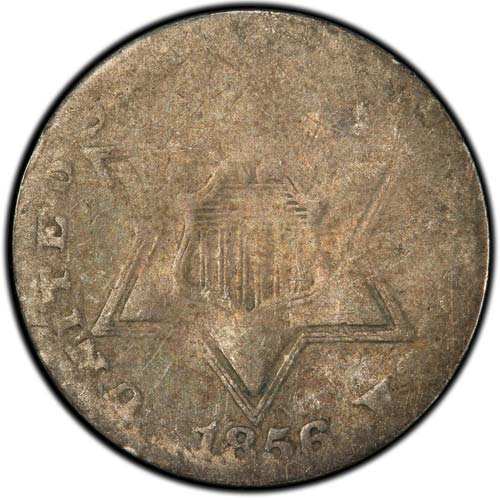
\includegraphics[width=0.45\linewidth]{images/3CentSil2-03o.jpg}
				\label{fig:cond0}
				\caption{Poor}
			\end{figure}
		\end{column}}
	\end{columns}
\end{frame}
\begin{frame}
	\setbeamertemplate{caption}{\raggedright\insertcaption\par}
	\frametitle{Conclusion}
	\begin{columns}[onlytextwidth]
		\begin{column}{.5\textwidth}
			\begin{figure}
				\includegraphics[width=.4\linewidth]{images/good.jpg}
				\label{fig:good}
				\caption{Uncased coin prediction rate 76\%}
			\end{figure}
			\begin{figure}
				\includegraphics[width=.4\linewidth]{images/bad.jpg}
				\label{fig:ok}
				\caption{Trouble with modern currency}
			\end{figure}
		\end{column}
		\begin{column}{.5\textwidth}
			\begin{figure}
				\includegraphics[width=.4\linewidth]{images/Better.jpg}
				\label{fig:bad}
				\caption{Cased prediction rate appears higher}
			\end{figure}
			\begin{figure}
				\includegraphics[width=.4\linewidth]{images/error.jpg}
				\label{fig:cond3}
				\caption{Confused by error printings}
			\end{figure}
		\end{column}
	\end{columns}
\end{frame}
\begin{frame}
	\titlepage
\end{frame}
\end{document}
